\section{Custom Instructions \weekDoran{2}}
	
	\subsection{General}
		In Qsys, custom instructions are assigned a unique index, called the selection index. In Assembly or in C/C++, this index is used to call the correct function.
		  
		\begin{itemize}
		  \item Can be visualised as being in parallel to the ALU.
		  \item Takes values from up to two source registers and writes result into destination register.
		  \item Appear as machine-generated assembly macros or C functions from the software perspective.
		  \item Increase system performance.
		\end{itemize}
		
	\subsection{Types of Custom Instructions}
	
		\begin{itemize}
		  \item Combinatorial
		  \item Multi-Cycle, synchronised by clock
		  \item Parametrised
		\end{itemize}
		
		\begin{table}[H]\centering
			\begin{tabular}{p{0.475\linewidth}p{0.475\linewidth}}
				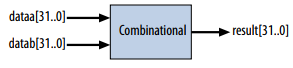
\includegraphics[scale=1]{./pictures/customInstCombinational.png}
					& 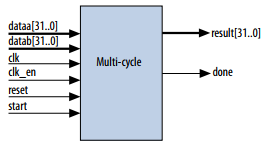
\includegraphics[scale=1]{./pictures/customInstMultiCycle.png}\\
			\end{tabular}
		\end{table}
		
	\subsection{Custom instruction Assembly Interface}
		This example shows a call to a custom instruction with the following parameters:
	
		\begin{table}[H]\centering
			\begin{tabular}{ll}
				Selection Index: 
					& 0\\
				Input (\texttt{dataa[31:0]}, \texttt{datab [31:0]}): 
					& Registers \texttt{R7}, \texttt{R8}\\
				Output (\texttt{result[31:0]}): 
					& Register \texttt{R8}\\
			\end{tabular}
		\end{table}
		
		\lstinputlisting[style=ASM, caption=Custom Instruction Assembly Interface]{./src/customInst.asm}

	\subsection{Custom instruction C/C++ Interface}
		\lstinputlisting[style=C, caption=Custom Instruction C/C++ Interface]{./src/customInst.c}